\DocumentMetadata{
  tagging=on,
  tagging-setup={math/setup={mathml-SE,mathml-AF},math/alt/use},
  pdfstandard=ua-2,
  pdfstandard=a-4f,
  lang=en-US
}
\documentclass[10pt]{article}
\usepackage{unicode-math}
%\usepackage{amsmath}
%\usepackage{amssymb}
\usepackage{multicol}
\usepackage{esdiff}
\usepackage{color}
\usepackage{ltablex}
\usepackage{mathtools}
\usepackage{enumitem}
\usepackage{listings}
\usepackage{hyperref}
\hypersetup{
pdftitle={From Laplace to Fourier},
pdfauthor={Bryan W. Lewis},
pdfkeywords={MAT 281 Diff Eq},%
}
\usepackage{cite}
\usepackage{authblk}
\usepackage{graphicx}
\usepackage{float}
\usepackage{fancyhdr}
\usepackage{geometry}
\geometry{
  margin=54pt,
  includeheadfoot
}
\pagestyle{fancy}
\renewcommand{\today}{\space\ifcase \month \or January\or February\or March\or April\or May \or June\or July\or August\or September\or October\or November\or December\fi,%
\space \number \year}
\rhead{\today}
\lhead{Differential Equations}
\pagenumbering{gobble}

\setlength{\parindent}{0pt}
\setlength{\parskip}{0.5em}

\begin{document}

\section*{From Laplace to Fourier}


\begin{minipage}[t]{0.5\textwidth}
\vspace{0pt}
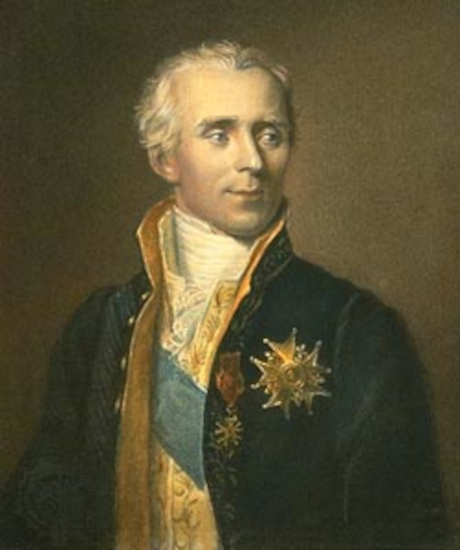
\includegraphics[width=0.9\textwidth,alt={Portrait of Laplace}]{laplace}
\\
\footnotesize{Portrait of Pierre-Simon Marquis de Laplace, 1749--1827}
\end{minipage}
\begin{minipage}[t]{0.5\textwidth}
\vspace{0pt}
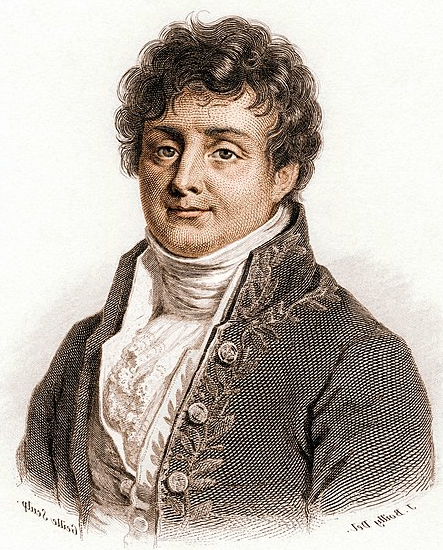
\includegraphics[width=0.87\textwidth,alt={Portrait of Fourier}]{fourier}
\\
\footnotesize{Portrait of Joe Fourier, 1768--1830}
\end{minipage}
\hrule

The Laplace transform can be used to simplify solving some differential
equations.  The transform essentially turns differential equations into
algebraic equations.  It's well-covered in our textbook here:
\url{https://www.jirka.org/diffyqs/html/laplace_section.html}.  Our textbook
also covers the Fourier transform in the context of partial differential
equations in this chapter:
\url{https://www.jirka.org/diffyqs/html/FS_chapter.html}.  You might not
realize it from reading our book, but the Laplace and Fourier transforms are
closely related---in fact, the Fourier transform \emph{is} a Laplace transform
with some restrictions applied.

These notes briefly:
\begin{enumerate}
\item Introduce the Laplace transform and show a few ODE examples.
\item Illustrate a few important properties of the Laplace transform.
\item Introduce the Fourier transform as a special case of the Laplace transform.
\end{enumerate}

\section*{The Laplace Transform}

Think of the Laplace transform $\mathcal{L}$ as a kind of function that takes one function $f$ as
input and returns another function $F$ as output. It's defined as:
\begin{equation}\label{laplace}
\mathcal{L}(f(t)) = F(s) = \int_0^\infty e^{-st}f(t)dt.
\end{equation}
The transform multiplies the input function $f$ by $e^{-st}$ and integrates from 
zero to infinity. And, the parameter $s$ of the new function is complex-valued
(real and imaginary components). This seems like it makes things more
complicated!

Although it seems complicated, in practice the Laplace transform can
dramatically simplify solving many differential equations---\textbf{in particular ones
that are not homogeneous}. Transforms are rarely integrated by hand. Usually we
simply look up the transforms of functions from a table or using software.
Table \href{https://www.jirka.org/diffyqs/html/laplace_section.html#lt_table}{6.1}
of our book lists some common transforms. The transforms in the table
are all invertible.

\subsection*{Example using the Laplace transform to solve an ODE}

The ode in this example is related to problem
\href{https://www.jirka.org/diffyqs/html/intfactor_section.html#intfactor_section-3-7}{1.4.9}
in our book---water flowing through two reservoirs. In particular, our
ODE shows flow in the lower reservoir under some simplifying assumptions.
It's a linear first-order, constant coefficient, non-homogeneous, ordinary differential equation:
\[
f'(t) + rf(t) = rqe^{-rt}, \qquad f(0)=0,
\]
for constants $r, q$ and time $t$.
There are many possible ways to solve for $f(t)$, including using an
\href{https://www.jirka.org/diffyqs/html/intfactor_section.html}{integrating
factor} or the Laplace transform. Let's use the Laplace transform! We'll use
capital $F(s)$ to be the transform of $f(t)$ to get:
\[
sF(s) - f(0) + rF(s) = \dfrac{rq}{s+r},
\]
and since $f(0)=0$, then:
\[
sF(s) + rF(s) = \dfrac{rq}{s + r}.
\]
Now we just solve for $F$ and then apply the inverse Laplace transform to get $f$!
\[
F(s) = \dfrac{rq}{(s + r)^2}.
\]
Applying the inverse Laplace transform yields:
\[
f(t) = rq t e^{-rt}.
\]

\section*{Properties of the Laplace transform}

\subsection*{Linearity}

The Laplace transform is just an integral and inherits linearity from that. In particular,
\[
\mathcal{L}(f + g) = \mathcal{L}(f) + \mathcal{L}(g) = F(s) + G(s).
\]

\subsection*{Time shifting}

\[
\mathcal{L}(f(t -T)) = e^{-sT}F(s).
\]

\subsection*{Convolution}

A \emph{convolution} of two functions $f$ and $g$ is defined to be:
\[
(f * g)(t) = \int_0^t f(u)g(t-u)du.
\]
This may seem like an odd operation but occurs naturally in many settings. In many
ways, convolution has product-like properties:
\begin{itemize}
\item[] $f*g = g*f$
\item[] $(f + g)*h = f*h + g*h$.
\item[] $(f * g) * h = f * (g * h)$.
\end{itemize}
Importantly, 
the Laplace transform of a convolution is the product of the Laplace transforms:
\[
\mathcal{L}(f*g) = F(s)G(s).
\]
The upshot is that if you ever have a product of transformed functions (like $F(s)G(s)$ above),
then the solution will be the \emph{convolution} of their inverse transforms.

Here is how that works. Say you wish to find the inverse Laplace transform of
$\frac{1}{s^2}\frac{1}{s+1}$:
\begin{enumerate}
\item Look up the inverse transform of $\frac{1}{s^2} = t$.
\item Look up the inverse transform of $\frac{1}{s+1} = e^{-t}$.
\item Now you know that the solution is the convolution of $t$ with $e^{-t}$, or $\int_0^t ue^{-(t-u)}du$.
\item Finish by evaluating $\int_0^t ue^{-(t-u)}du = e^{-t} + t - 1$ (for instance with integration by parts!).
\end{enumerate}

\subsection*{Dirac's delta function}

Named for Paul Dirac, the delta function, or $\delta$ is not exactly a normal function. Imagine a box with area
one centered at 0 on the x-axis. Such a box between, say, $-\frac{1}{2} \le x \le \frac{1}{2}$ would have
height 1. But between $-\frac{1}{4} \le x \le \frac{1}{4}$ the height of the box would have to be 2 to
still have area equal to 1. Think of the delta function as the limit of those boxes as the $x$-values approach
zero. The function is essentially zero everywhere and infinite when $x=0$.

The Laplace transform of the delta function is 1, $\mathcal{L}(\delta(t)) = 1$.
Solving a differential equation for \emph{impulse response} means setting the
ODE equal to $\delta(t)$.  See
\href{https://www.jirka.org/diffyqs/html/diracdelta_section.html#diracdelta_section-5-3}{Example
6.4.2} for a good example.


\section*{From Laplace to Fourier...}

You may have noticed that integration in the Laplace transform is usually defined from 0 to $\infty$.
It's also possible to define a bi-infinite (also called bi-lateral) transform:
\begin{equation}\label{bilaplace}
\mathcal{L}(f(t)) = F(s) = \int_{-\infty}^\infty e^{-st}f(t)dt.
\end{equation}
This version of the transform shares many of the same properties with Equation\eqref{laplace}.
It accounts for the entire history of a signal, not just from time greater than zero.

Earlier we mentioned that the parameter $s$ of the transformed function is complex-valued---so
it looks like $\alpha + \beta i$ where $i=\sqrt{-1}$ is the imaginary unit.
The real part $\alpha$ acts as a ``damping'' or ``growth'' factor.
The imaginary part $\beta$ deals with oscillation.
If we restrict
that parameter so the real part $\alpha=0$, then $s=\beta i$ is a purely imaginary number
and the transform is focused on steady-state oscillation.
That's the Fourier transform! Thus, the Fourier transform is a special case of the Laplace
transform.

Finally, assume that the function $f$ is periodic with period $T$---that is the
function repeats itself over interval length $T$.  For the transform to be
consistent with this periodicity, the kernel $e^{-st}$ must satisfy the same
boundary conditions as the function itself.
Since $f(t) = f(t + T)$, that means that $e^{-st} = e^{-s(t + T)} = e^{-st}e^{-sT}$.
That can only be true if $e^{-sT} = 1$, which means that $-sT$ is a multiple of $2\pi$
because of Euler's formula:
$e^{\beta t i} = \cos(\beta t) + i\sin(\beta t).$
Therefore,
\[
-sT = -i(2\pi n)\qquad\mbox{for }n=0, \pm 1, \pm 2, \ldots.
\]
Solving for $s$ shows that rather than a continuous line along the imaginary axis, $s$ takes on
discrete points:
\[
s_n = i\left(\dfrac{2\pi n}{T}\right).
\]
That means that the corresponding Fourier transform is
\begin{equation}\label{cfourier}
F(s_n) = \int_{-\infty}^\infty e^{-it\frac{2\pi n}{T}}f(t)dt.
\end{equation}


\subsection*{The Fourier Series}

Notice that Equation\eqref{cfourier} is defined on discrete points along the imaginary ($i$) axis.
With some effort we will show in future notes that the inverse transform associated
with Equation\eqref{cfourier} reduces to a series:
\begin{equation}\label{fourier}
f(t) = \sum_{-\infty}^{\infty}\dfrac{1}{T}F_T\left(i\dfrac{2\pi n}{T}\right)e^{i\frac{2\pi n}{T}t},
\end{equation}
where 
\[
F_T(s_n) = \int_0^T f(t) e^{-s_n t}dt
\]
is the transform of $f(t)$ over one period. This is the usual Fourier series definition
of the function $f$.
The values
\[
c_n = \dfrac{1}{T}F_T\left(i\dfrac{2\pi n}{T}\right)
\]
are called the Fourier coefficients of $f$.


\subsection*{The Discrete and Fast Fourier Transforms}

Functions (signals) are often measured over discrete points in
time to produce a finite sequence of values.  The \emph{discrete fourier
transform} (DFT) converts that finite sequence into another finite sequence of
the same length that represent the Fourier coefficients (frequency components)
of the signal. When sampled at equally-spaced points, the DFT represents a trig
polynomial that interpolates the signal at those points.

The DFT is typically computed using the \emph{fast fourier transform} (FFT), a
remarkably-efficient algorithm developed by Cooley and Tukey in 1965---but
later discovered to be originally invented by Gauss in 1805. The FFT and its
variations is an enabling technology for much of modern signal processing. Its
importance is hard to over-state.





\end{document}
